
\section{LLVM}
The LLVM Project \cite{llvm} is a collection of modular and reusable compiler toolchain technologies. It is built around an intermediated representation called LLVM-IR, and provides a set of APIs to interact with it. LLVM provides an optimizer that works on the intermediate representation, and also several code generation helpers that allow to target all the main hardware architectures.
\subsection{LLVM-IR}
The LLVM-IR is a language that resembles a generic assembly language, while also providing some high level features such as unlimited registers, explicit stack memory allocation and pointer deferentation.
This allows LLVM-IR to be both the ideal target for high-level language developers, that do not have to worry about architecture specific details, and also the ideal source language for compiler back-end developers, that have to implement only a translator from LLVM-IR to their target architecture's assembly language, without worrying about high-level language features. \par
The LLVM-IR is accesible in three formats: in-memory represantation, that allows manipulation through the LLVM APIs, binary format, used by many LLVM tools, and the human-readable textual format, that can also very conveniently be parsed by means of the APIs.

\subsection{SSA and Phi nodes}
The LLVM-IR is by definition in SSA (Static Single Assignment) form. The SSA form requires a variable to be assigned only once, and requires every variable to be defined before its uses. It is called static because it does not take into account dynamic (related to the program's runtime) considerations. For instance, an assignment in a loop counts always as one assignment, even if at runtime it will be performed several times.\newline
----esempio \newline
It is always clear which definition to use, unless a basic block has multiple predecessors. In that case it is necessary to add phi nodes that carry the information to disambiguate the uses at runtime.\newline
----esempio
\newline

\subsection{Class hierarchy}
The class hierarchy defined in the LLVM APIs consists of hundreds of classes, a complete and exhaustive view is given by the LLVM Doxygen Documentation. The main components of the hierarchy are:
\begin{itemize}
\item Module: the entire program/compile unit. Contains the global values of the program: mainly the global variables and the functions.
\item Function: a function in the compile unit, contains mainly a set of arguments and it's control flow graph in the form of a set of basic blocks.
\item Basic Block: a set of instructions with no branches between them.
\item Instruction: An instruction of the IR.
\end{itemize}
Another key class in the LLVM class hierarchy is the Value class. It represents anything that has a type and can be used as an operand to an instruction: function arguments, constants, instructions, basic blocks and functions are all Values.
A Value also carries information of what other Values it uses, and what other Values use it.

\subsection{LLVM Metadata}
The LLVM-IR allows metadata to be attached to Instructions, Functions, Global Variables or  Modules. Metadata can convey extra information about the code to the optimizers and code generator.
The main use of metadata is debug information, but they may also carry information about loop boundaries or other assumption that are useful during the various stages of the compilation process. \par
Metadata can either be a simple string attached to an instruction, or they can be a Metadata Node (MDNode). MDNodes can reference each other and are specified by other classes in the LLVM APIs. See section \ref{sec:llvm-dbg} or the LLVM Language Reference \cite{llvm-langref} for more details.

\subsection{LLVM Passes\label{sec:llvm-passes}}
LLVM passes are where most of the interesting parts of the compiler exist. Passes perform the transformations and optimizations that make up the compiler, they build the analysis results that are used by these transformations, and they are, above all, a structuring technique for compiler code. \par
Passes are categorized in two ways: by the granularity at which they operate, and by the fact that they perform changes on the module or not. \newline
By the first categorization, passes are identified as:
\begin{itemize}
\item Module Passes: operate on an entire Module.
\item Function Passes: operate on a single Function.
\item Loop Passes: operate only on loops.
\item Region Passes: operate on subsets of Basic Blocks of a Function, with a single entry point and a single exit point.
\end{itemize}
By the second categorization, passes are identified as:
\begin{itemize}
\item Analysis Passes: passes that only perform an analysis of the given entity, without modifying it. 
\item Transformation Passes: passes that may modify the given entity. They exploit the results of the Analysis Passes, often (but not only) in order to perform optimizations: the may add, remove, move or replace instructions and basic blocks, with the ultimate goal of improving performances or reduce the size of the binary.
\end{itemize} \par 
Passes may depend on other passes, for instance a pass that performs an optimization may require the results of a pass that performs a specific analysis.
They are therefore handled by a Pass Manager that schedules the passes, ensuring that all the dependencies for a pass are met before executing it. 

\section{How LLVM handles debug information\label{sec:llvm-dbg}}

\subsection{Metadata classes}
\subsection{Transformation passes guidelines}
As we've seen in section \ref{sec:llvm-passes}, during the compilation a module may undergo some changes: instructions may be removed, moved, merged together, and replaced with new instructions, all in order to improve the performances of the resulting program. \par 
This transformations have the side effect of obfuscating the correspondence between source code and binary code: before the optimization occurs, debug information provide a very clear, one to many relation between source location and LLVM-IR instructions. But as the module progresses into the optimization pipeline, it becomes more and more difficult to maintain this relation. \par
In general it is not possible to map unambiguously source locations to optimized code, but the LLVM project provides a set of guidelines that specify how to correctly update debug info when implementing transformation passes \cite{llvm-guidelines}. \newline
Here we provide a short summary of such guidelines \footnote{Provided at a speech and the 2020 LLVM Conference by Adrian Pranti and Vedant Kumar}, highlighting some behaviors that, even when following them, lead to a loss of information regarding source-binary mapping. This behaviors are not bug or mistakes of the people who provided the guidelines, but are instead related to the fact that they want to provide a debugging experience as close as possible to the one that a user would have while debugging the unoptimized code. \par 
The guiding principles for a developer that wants to update debug info are the following:
\begin{enumerate}
\item Do not provide misleading information: a developer should not speculate, and providing no information is better than providing wrong information that may lead a developer to wrong considerations about the behavior of his program.
\item Provide as much information as possible: when it's not misleading, information should be preserved. 
\end{enumerate}
In order to achieve this, when choosing what do to with the debug information of a given instruction, a developer has three alternatives:
\begin{itemize}
\item Preserve the original location.
\item Merge two locations: two debug locations can be merged together. Locations merge is performed by computing the intersection of the two locations: the resulting location will contain only the information that the original two had in common.
\item Delete the location.
\end{itemize}
Locations can be safely preserved when the modified instruction either remains in the same basic block, or its basic block is folded into a predecessor that branches unconditionally. For instance, an optimization the replaces the instruction {\fontfamily{qcr}\selectfont add x x} with a binary shift to the left ({\fontfamily{qcr}\selectfont shl x 1}) can safely keep the location of the original add. \par 
Location should be merged when two instructions are replaced with a new instruction. An example of that is figure \ref{fig:merge}, in which the two stores can be merged into a new one, inserted in the exit basic block: the new instruction effectively replaces the original two, and therefore its location will be the merged location of the old ones. \par
\begin{figure}
\centering
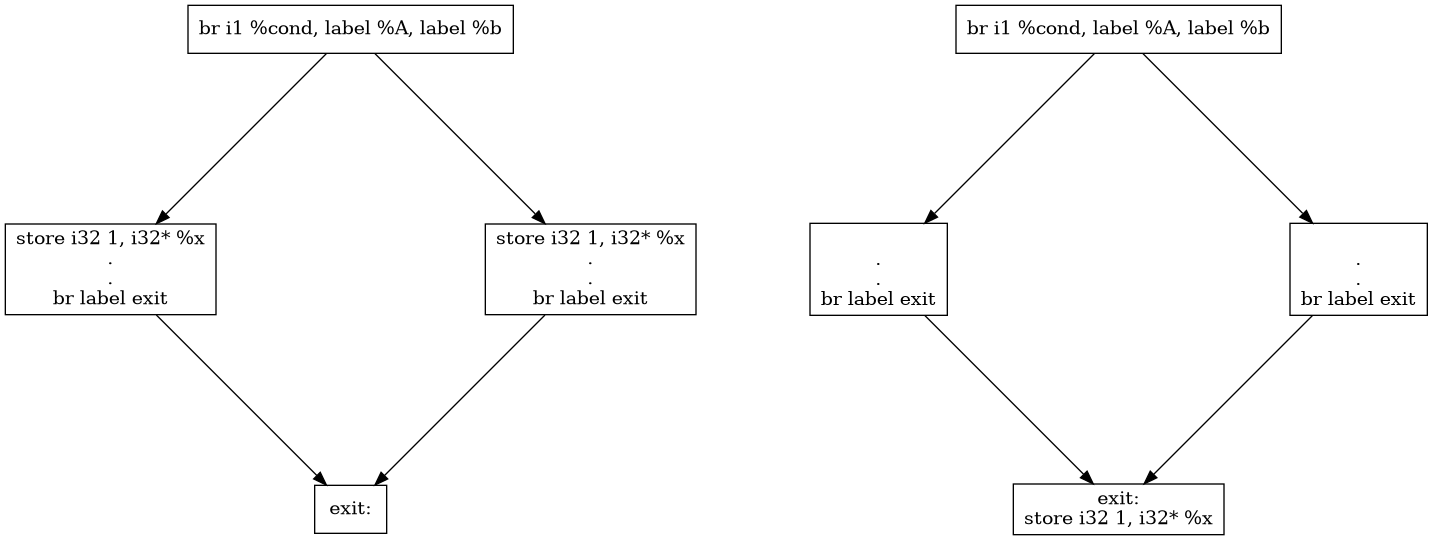
\includegraphics[scale=0.3]{chapter-2/merge.png}
\caption{Example of optimization with merged debug location}
\label{fig:merge}
\end{figure}
In all the cases in which the previous rules do not apply, locations should be dropped. In particular, they should be dropped whenever an instruction is moved from a basic block with multiple predecessors, to one of the predecessors. This is done to avoid situations in which, while debugging, the program seems to have taken a branch in a conditional, while the actual conditions are not the one that would have resulted in the branch being taken. \par 
Dropping locations and merging locations is a very reasonable course of action when dealing with debugging: they lead to a debugging experience that is as close as possible to the not optimized one. But they also lead to a loss of information in the source-binary mapping: when two locations are merged, we will most likely lose the information on the original source code lines, as they probably will not be equal, and when a location is dropped we will of course lose the information it carried.\par
We have therefore developed a methodology that allows to propagate debug locations through the optimization pipeline, while also bringing to the developers a view of the optimizations performed on their program, so that they can understand how it has been optimized by the compiler.

\section{Program Instrumentation}
Instrumenting a program means to insert additional code that was not originally in the program's source, typically in order to produce additional information (regarding some functional or non functional properties) during the program's runtime. It can be performed directly on the source code, on the executable binary, or during the compilation.
An example of instrumentation are the many sanitizers that are part of the LLVM project, they make runtime checks about memory and thread safety. \par 
LLVM provides some helper classes to perform instrumentation on an IR Module, and in general a user may define his own transformation pass that inserts new code into the program being compiled.
\par
Instrumentation often introduces a performance overhead, due of course to the fact that more instructions are executed while the program is running, so it is usually performed only during the development stage of an application.


\section{Debugging}
A debugger is a computer program used to test and debug other programs. It allows a programmer to run the target program in controlled conditions, pause the program's execution, check the state of variables and more.

\subsection{Debug information}
The main functionality of a debugger, over which more advanced features can be built, are setting break points and accessing the content of a variable defined in the source code. \newline 
This is achieved by means of debug information: information stored by the compiler in the program's executable, with the purpose of providing a correspondence between source level entities (variable, source code locations, data types) and low level entities (assembly instructions and memory locations). \par
The format used to store them may vary with the compiler/operating system used, but the stored information are mainly:
\begin{itemize}
\item Definition of the data types employed in the program and their layout in memory, both language-defined (eg. int, float, unsigned in C) or user defined (eg. C structs or C++ classes). 
\item Mapping between variables defined in the source code and memory locations in which they are stored. This allows a debugger to output the value of a variable given its name.
\item Mapping between source code locations and assembly instruction. This allows the debugger to pause the program's execution when a given source code location is reached.
\end{itemize}
These information are useful not only for debugging purposes, they may also be employed by any other tool that requires a mapping between source code and binary executable, such as a profiler or a test coverage tool, that may be able to annotate the source code with the information that they have gathered.

\subsection{DWARF format}

The DWARF format \cite{dwarf} is a debugging file format used by many compilers and debuggers to support source-level debugging. It is designed to be extensible with respect of the source language, and to be architecture and operating system independent. \par
The main data structure used to store debug information is the DIE (Debug Information Entry). DIEs are used to describe both data types and variables, and can reference each other creating a tree structure. \par
Another data structure that is very useful for our purposes is the Line Number Table: it contains the mapping between memory addresses of the executable code, and the source line corresponding to those addresses.\newline
Each row of the table contains the following fields:
\begin{itemize}
\item Address: the program counter value of a machine instruction.
\item Line: the source line number.
\item Column: the column number within the line.
\item File: an integer that identifies the source file.
\item Statement: boolean indicating if the current instruction is the beginning of a statement.
\item Block: boolean indicating if the current instruction is the beginning of a basic block.
\end{itemize}
And other fields that are described in the DWARF documentation.


